\documentclass[12pt,singleside,a4paper]{article}
\usepackage{graphicx}
\usepackage{epsfig}
\usepackage{cite}
\usepackage{geometry}
\usepackage{float}
\usepackage{subfig}
\usepackage{comment}
\geometry{left=20mm,right=20mm,top=20mm,bottom=50mm}
\pagestyle{plain}
\pagestyle{plain}
\usepackage[demo]{graphicx}
\usepackage{babel,blindtext}

 \title{Software Documentation For Quartus Prime and ModelSim}
\author{Chethan T Bhat, Ritvik Tiwari, Karthik A Shet, Ajay Chaudari}
\date{May 2020}
\renewcommand*\contentsname{Table of Content}
\begin{document}

\maketitle
\newpage
\tableofcontents
\newpage
\pagenumbering{arabic}


%\-------------------------------------------------------------------------------
\begin{sloppypar}
\section{What are Quartus and ModelSim?}
\end{sloppypar}

Intel Quartus Prime is programmable logic device design software by Intel; prior to Intel's acquisition of Altera the tool was called Altera Quartus Prime, earlier Altera Quartus II. Quartus Prime enables analysis and synthesis of HDL designs, which enables the developer to compile their designs, perform timing analysis, examine RTL diagrams, simulate a design's reaction to different stimuli, and configure the target device with the programmer. Quartus Prime includes an implementation of VHDL and Verilog for hardware description, visual editing of logic circuits, and vector waveform simulation.

ModelSim is a multi-language HDL simulation environment by Mentor Graphics, for simulation of hardware description languages such as VHDL, Verilog and SystemC, and includes a built-in C debugger. ModelSim can be used independently, or in conjunction with Intel Quartus Prime, Xilinx ISE or Xilinx Vivado. Simulation is performed using the graphical user interface (GUI), or automatically using scripts.
\\


%\-------------------------------------------------------------------------------
\section{Installing Quartus and ModelSim}
\par In this part of the guide we will walk through the process of installing the software Quartus Prime Lite Edition Version 19.1\\
\par System Requirement: 
\begin{enumerate}
    \item A full installation of the Intel FPGA Complete Design Suite v19.1 requires approximately 14GB of available disk space on the drive or partition where you are installing the software.
    \item Recommended Physical RAM requirement is more than 2GB.
\end{enumerate}
\par If you are running any type of antivirus software, you can temporarily disable the software during the Quartus Prime software download and installation process to avoid unnecessary issues.
\par On the Download Page select the edition as lite and select version as 19.1.
Also select the desired operating system. We selected window for further installation. 
\begin{figure}[H]
\centering

\includegraphics[width=14cm,height=104cm,keepaspectratio]{InstallationImages/Version.png}
\end{figure}
%----
\subsection{Download using Complete Software Package}
\begin{figure}[H]
\centering
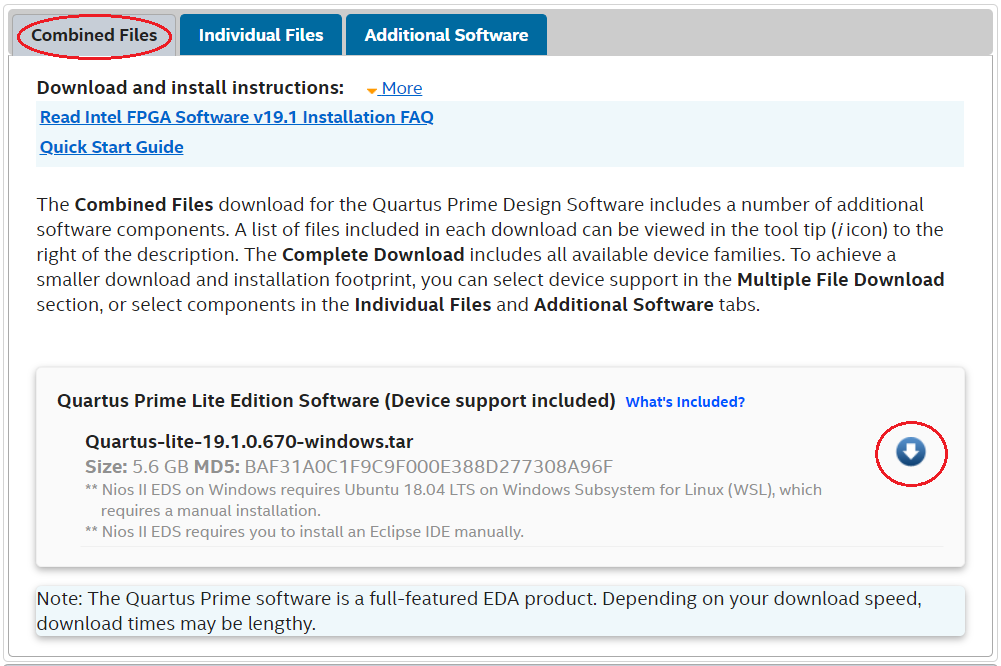
\includegraphics[width=14cm,height=104cm ,keepaspectratio]{InstallationImages/CombinedFiles.png}
\end{figure}
\begin{enumerate}
    \item The Combined Files download includes a number of additional software components. This file provides device support for various device families.
    \begin{enumerate}
        \item Arria II device support. 
        \item Cyclone IV device support. 
        \item Cyclone 10 LP device support.  
        \item Cyclone V device support.
        \item MAX II, MAX V device support. 
    \end{enumerate}
    
    \item After download is done on your local machine, extract all of the files to the same directory using WinZip or any other software. 
        
\end{enumerate}

\subsection{Download using Individual Software Package }
\begin{figure}[H]
\centering
\includegraphics[width=14cm,height=104cm ,keepaspectratio]{InstallationImages/IndividualFiles.png}
\end{figure}
\begin{enumerate}
    \item In Individual Files download, download both Quartus Prime lite edition and ModelSim, you also need to download files to get support for a particular device family.
    \item Select from the below option which are necessary.
    \begin{enumerate}
        \item Arria II device support. 
        \item Cyclone IV device support. 
        \item Cyclone 10 LP device support.  
        \item Cyclone V device support.
        \item MAX II, MAX V device support. 
    \end{enumerate}
    \item Download Cyclone IV device support as Intel DE0-Nano uses Altera Cyclone IV, it will also support other device from the same family. 
        
\end{enumerate}

\subsection{Installation after Download}
\begin{enumerate}
    \item After Download necessary files extract them in a single folder and click on the QuartusLiteSetup and allow 
    \begin{figure}[H]
        \centering
        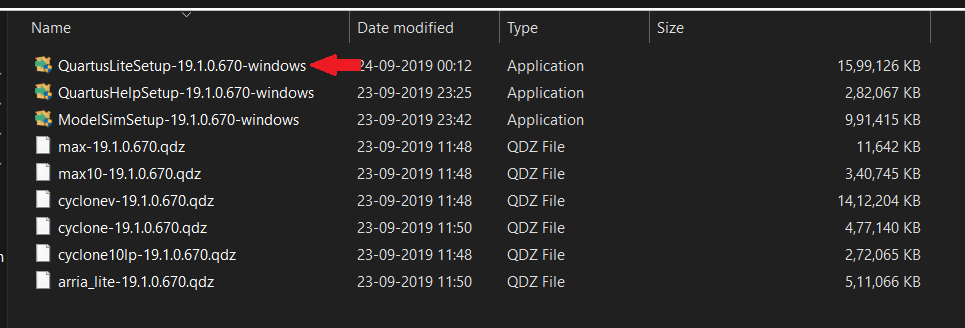
\includegraphics[height = 14cm, width =14cm,keepaspectratio]{InstallationImages/Setup.png}
        \end{figure}
    \item Click on next to start with the installation.
    \begin{figure}[H]
        \centering
        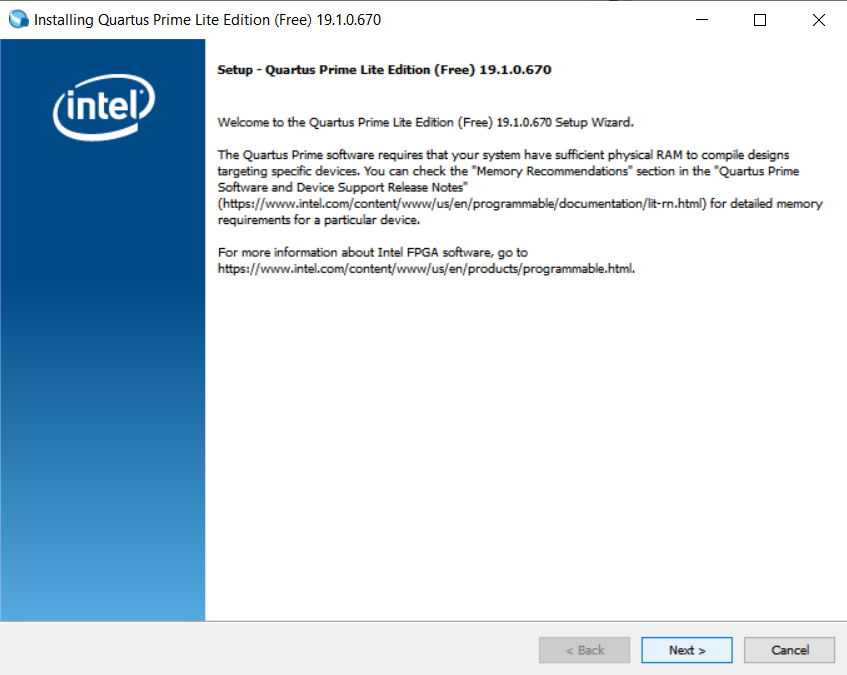
\includegraphics[height = 14cm, width =14cm,keepaspectratio]{InstallationImages/Next1.png}
        \end{figure}
    \item Click on agree with terms and condition and proceed
    \begin{figure}[H]
        \centering
        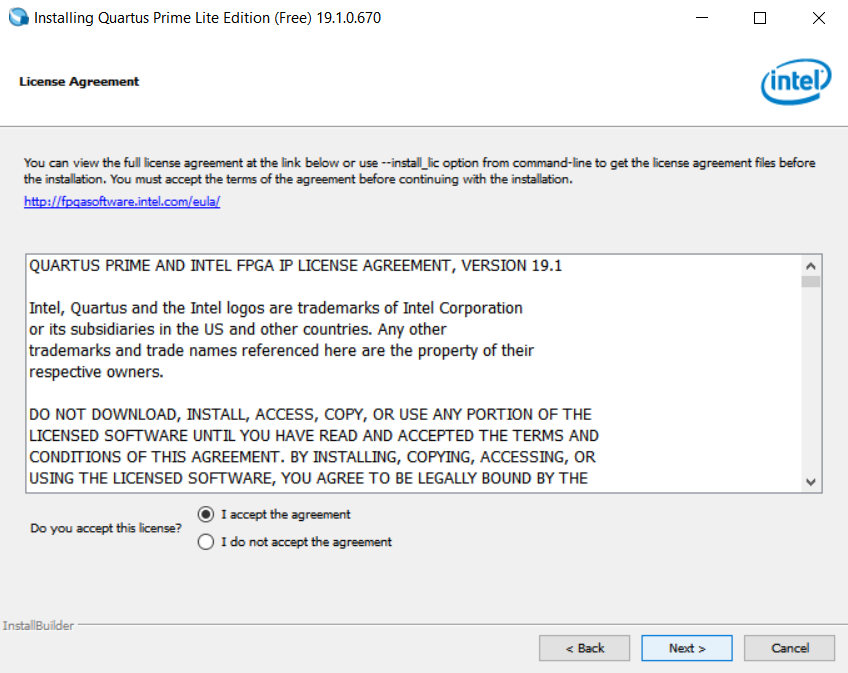
\includegraphics[height = 12cm, width =12cm,keepaspectratio]{InstallationImages/Next2.png}
        \end{figure}
    \item Enter the path where u need the software to be installed 
    \begin{figure}[H]
        \centering
        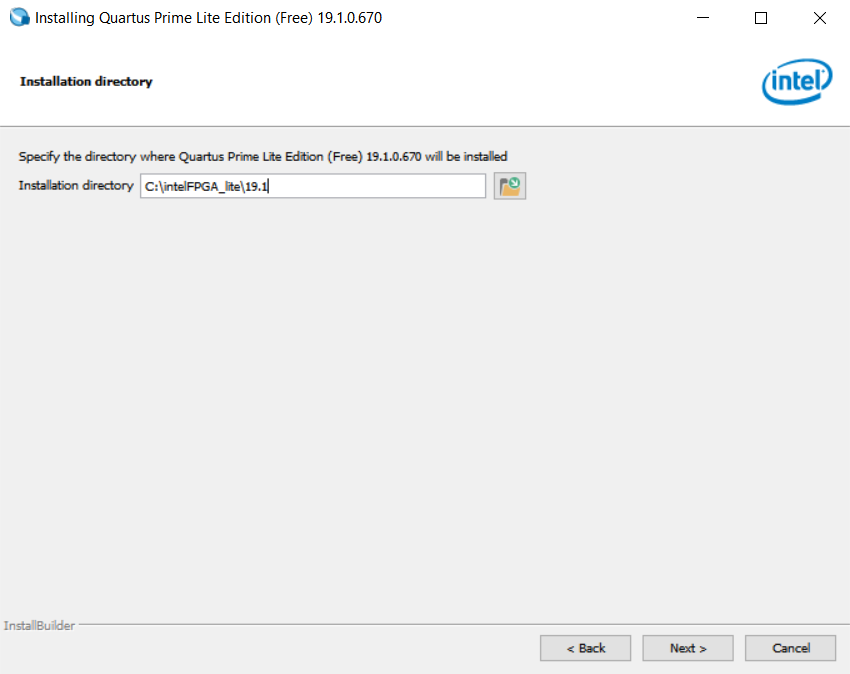
\includegraphics[height = 12cm, width =12cm,keepaspectratio]{InstallationImages/Next3.png}
        \end{figure}
    \item After this the installation starts and may takes some time to complete during this time ModelSim and QuartusHelp will also get installed
    \item Copy the below file and paste it in the 
   C:/intelFPGA\_lite/19.1/modelsim\_ase/win32aloem folder to get support of the device families while creating project
    \begin{figure}[H]
        \centering
        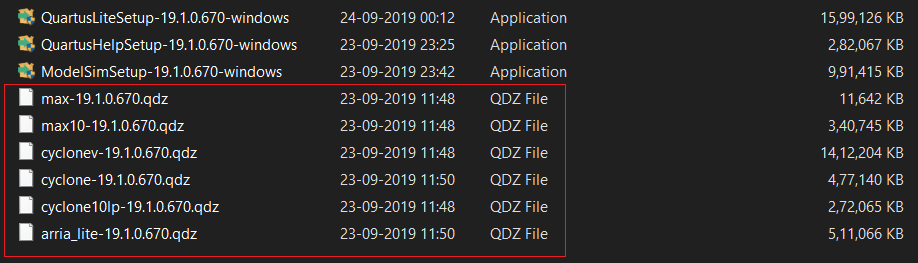
\includegraphics[height = 14cm, width =14cm,keepaspectratio]{InstallationImages/Next4.png}
        \end{figure}
\end{enumerate}


%\-------------------------------------------------------------------------------
\section{Getting started with Quartus prime}
\subsection{Creating a new project}
\textbf{Step 1} : Open the Quartus Prime Software

\noindent \textbf{Step 2} : Click on File and then click on New Project Wizard. Alternatively, New project wizard \hspace*{37pt} can be opened from the home tab that is seen when quartus is opened.
\begin{figure}[H]
\centering
\includegraphics[height = 11cm, width = 18cm,keepaspectratio]{Step_2.jpg}
\end{figure}
\newpage
\noindent \textbf{Step 3}: Click Next on the Dialog Box and select the directory in which the project is to be \hspace*{37pt} saved. Give the project name and click on next.
\begin{figure}[H]
\centering
\includegraphics[height = 10cm, width = 18cm]{Step_3.jpg}
\end{figure}

\noindent \textbf{Step 4} : Choose a project Template if its present, else choose empty project.
\begin{figure}[H]
\centering
\includegraphics[height = 9.5cm, width = 18cm]{Step_4.jpg}
\end{figure}

\noindent \textbf{Step 5} :Add all the necessary files(if any) and click on next.
\begin{figure}[H]
\centering
\includegraphics[height = 8cm, width = 18cm]{Step_5.jpg}
\end{figure}

\noindent \textbf{Step 6} : Choose the fpga device that is being used. Select the family and choose the chipset \hspace*{39pt} from the list or search for a specific name using the filter provided.If the device being \hspace*{39pt} worked on is a development kit, then click on the boards tab and choose the relevant \hspace*{39pt} kit
\begin{figure}[H]
\centering
\includegraphics[height = 10.5cm, width = 18cm]{Step_6.jpg}
\end{figure}

\noindent If the device being  worked on is a development kit, then click on the boards tab and choose the relevant kit
\begin{figure}[H]
\centering
\includegraphics[height = 10cm, width = 18cm]{Step_6_1.jpg}
\end{figure}

\noindent \textbf{Step 7}: Select the tools used in the project. For simulation, choose ModelSim-alterra. Also \hspace*{39pt} choose a suitable format(verilog, VHDL or SystemVerilog)
\begin{figure}[H]
\centering
\includegraphics[height = 9cm, width = 18cm]{Step_7.jpg}
\end{figure}

\noindent \textbf{Step 8} :Review the information and click on finish to successfully create a Project
\begin{figure}[H]
\centering
\includegraphics[height = 11.5cm, width = 18cm]{Step_8.jpg}
\end{figure}

\newpage
\subsection{Creating new files in the project}
\begin{enumerate}
\item Verilog/VHDL File
\newline
\newline
\textbf{Step 1}: Click on file and then click on new
\begin{figure}[H]
\centering

\includegraphics[height = 11.5cm, width = 16cm]{img1.png}
\end{figure}
\newpage
\noindent \textbf{Step 2} :Select the file type from drop down menu i.e either verilog or VHDL
\begin{figure}[H]
\centering
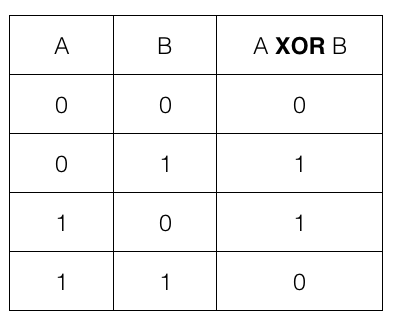
\includegraphics[height = 9cm, width = 15cm]{img2.png}
\end{figure}
\noindent \textbf{Step 3}:Write down your verilog or VHDL code (For demonstration we have used a simple 8 bit up-counter code)
\begin{figure}[H]
\centering
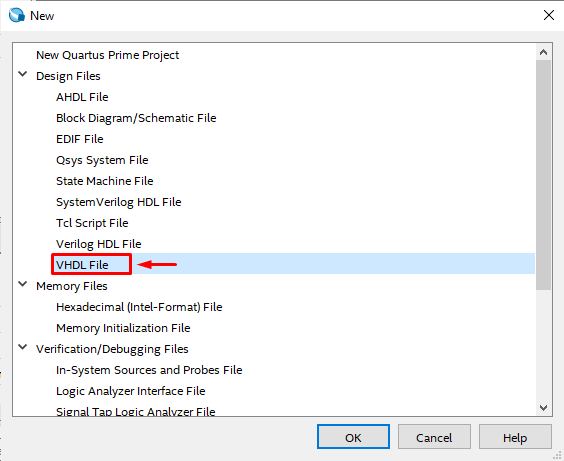
\includegraphics[height = 9cm, width = 15cm]{img3.png}
\end{figure}

\newpage
\noindent \textbf{Step 4} :After completing the code click on file and then select save as
\begin{figure}[H]
\centering
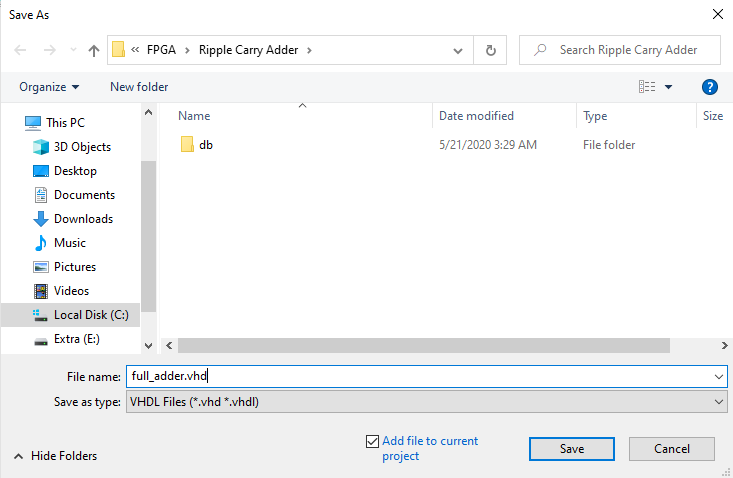
\includegraphics[height = 9cm, width = 15cm]{img4.png}
\end{figure}
\noindent \textbf{Step 5}:Enter the name of file ( it should be similar to module/entity name), select the file type and then click on save
\begin{figure}[H]
\centering
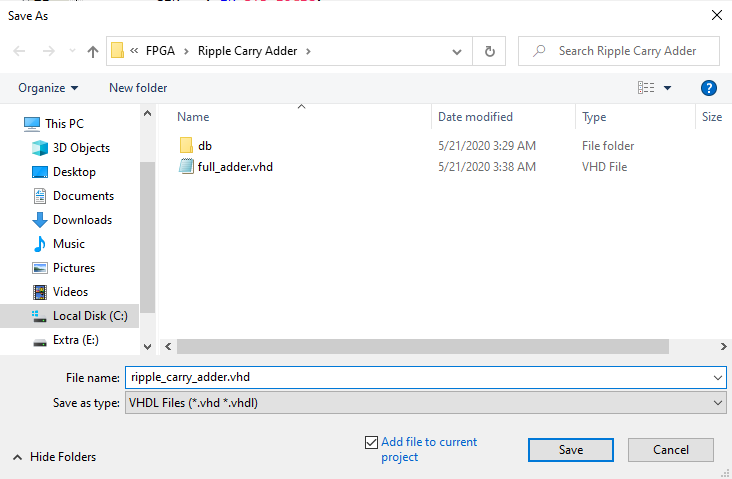
\includegraphics[height = 9cm, width = 15cm]{img5.png}
\end{figure}
\newpage
\item Block Diagram File
\newline
\newline
\textbf{Step 1}: Click on file$\rightarrow$new and select Block Diagram/Schematic File from the drop down menu
\begin{figure}[H]
\centering
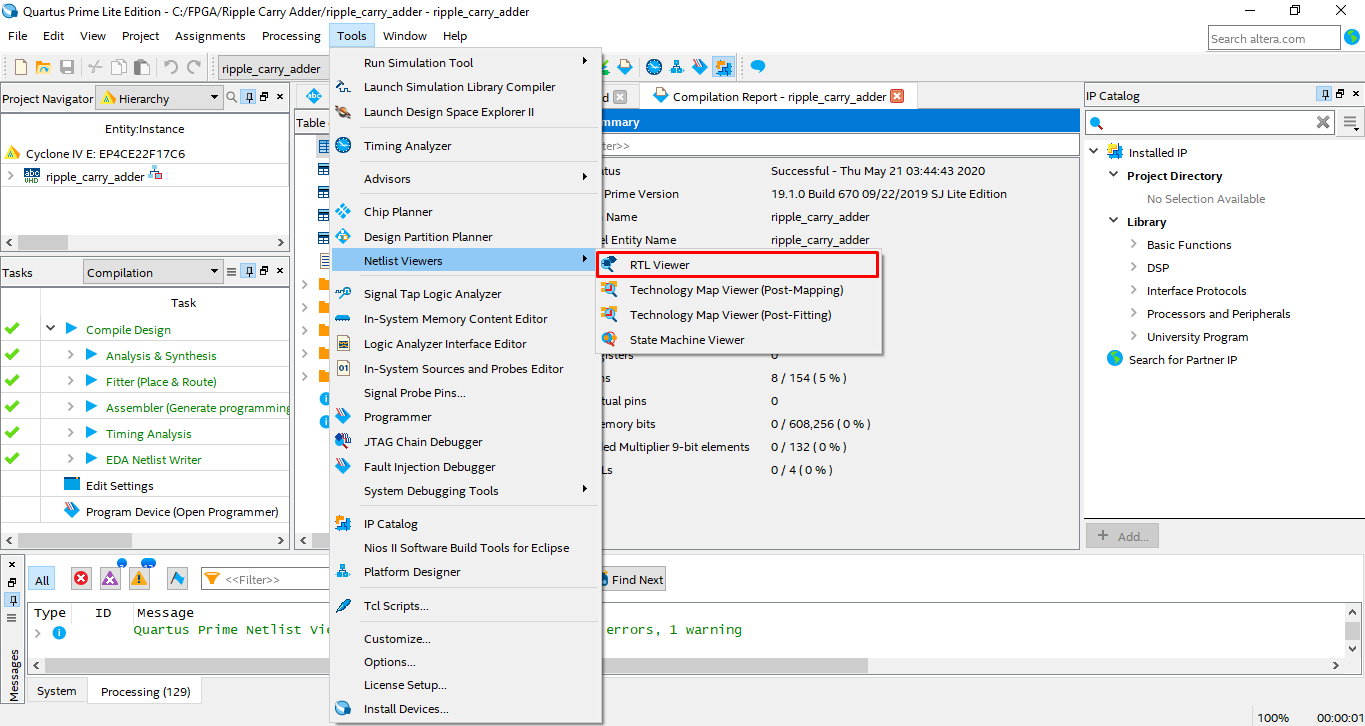
\includegraphics[height = 9cm, width = 16cm]{img for 3.2/img9.png}
\end{figure}
\noindent \textbf{Step 2}: Create symbol files for your block diagram. First of all go to your vhdl/verilog code. Then, Go to file$\rightarrow$Create/Update$\rightarrow$Create symbol files for current file
\begin{figure}[H]
\centering
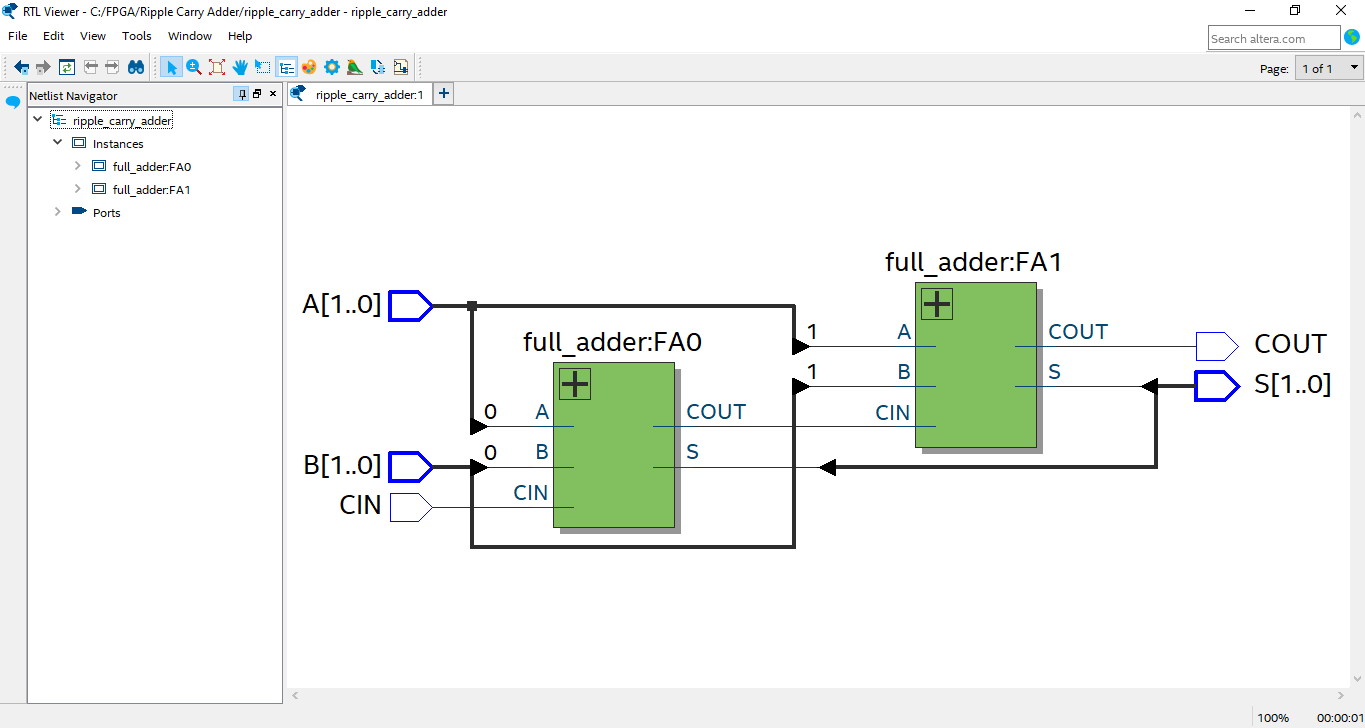
\includegraphics[height = 9cm, width = 15cm]{img for 3.2/img10.png}
\end{figure}
\noindent \textbf{Step 3}:Import your symbol files in your block diagram. Click on the symbol tool
\begin{figure}[H]
\centering
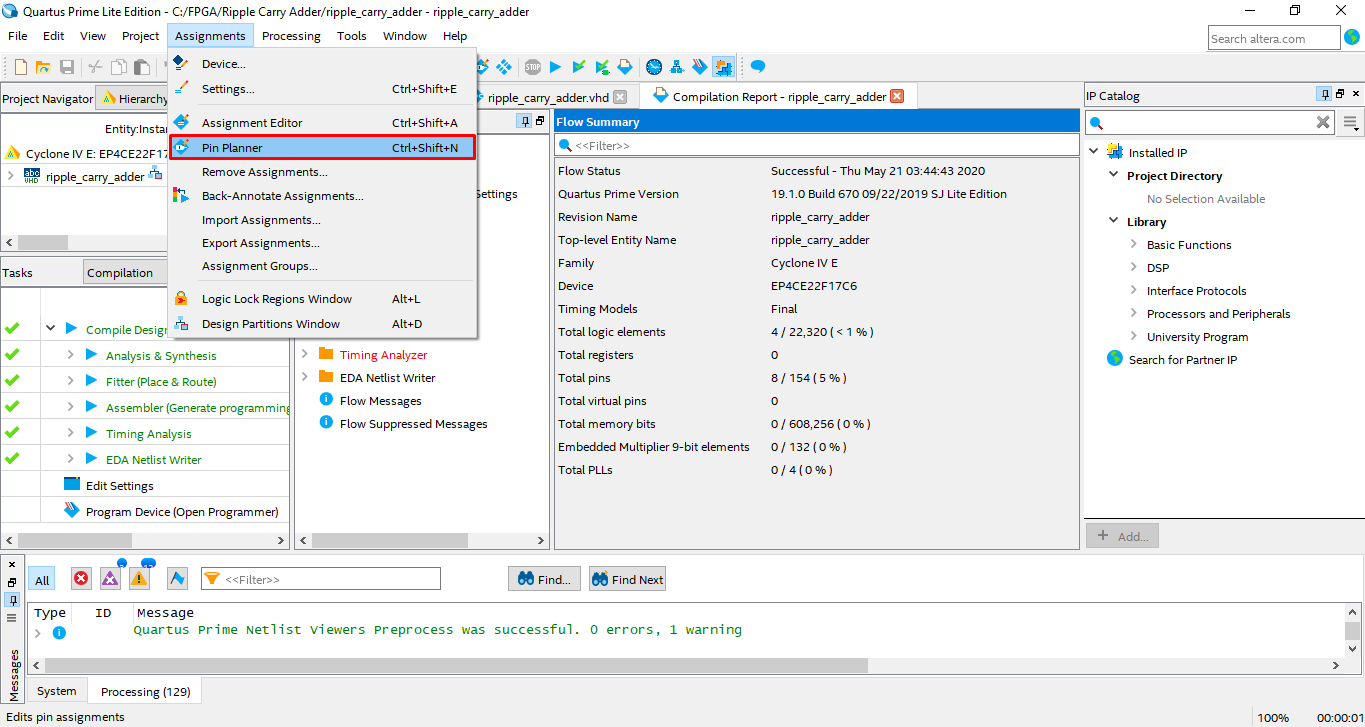
\includegraphics[height = 10cm, width = 15cm]{img for 3.2/img11.png}
\end{figure}
\noindent \textbf{Step 4}:Now, select your project and click on OK. You can place the symbol anywhere in your layout.
Note: You can place many duplicates of the same symbol by clicking repeatedly, until you press esc.
\begin{figure}[H]
\centering
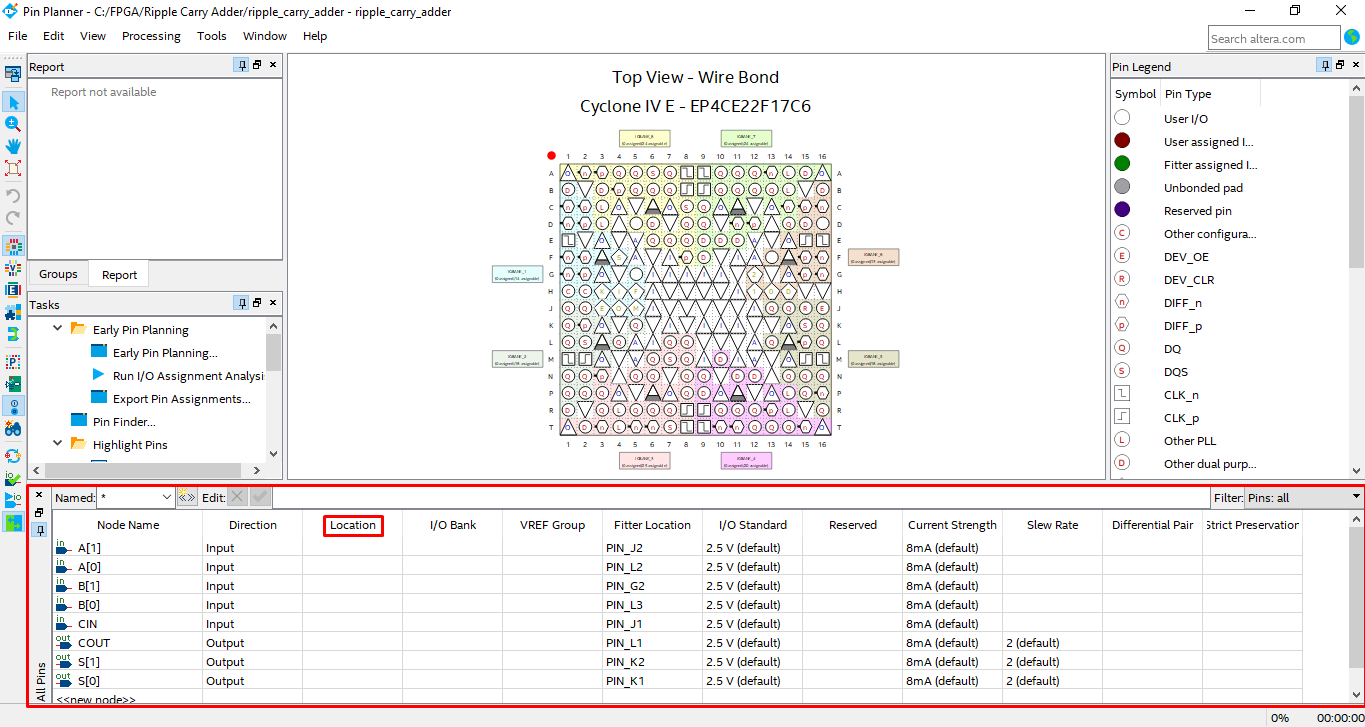
\includegraphics[height = 9cm, width = 15cm]{img for 3.2/img12.png}
\end{figure}
\noindent \textbf{ Step 5}:You can use the Orthogonal Node Tool for making connections
\begin{figure}[H]
\centering
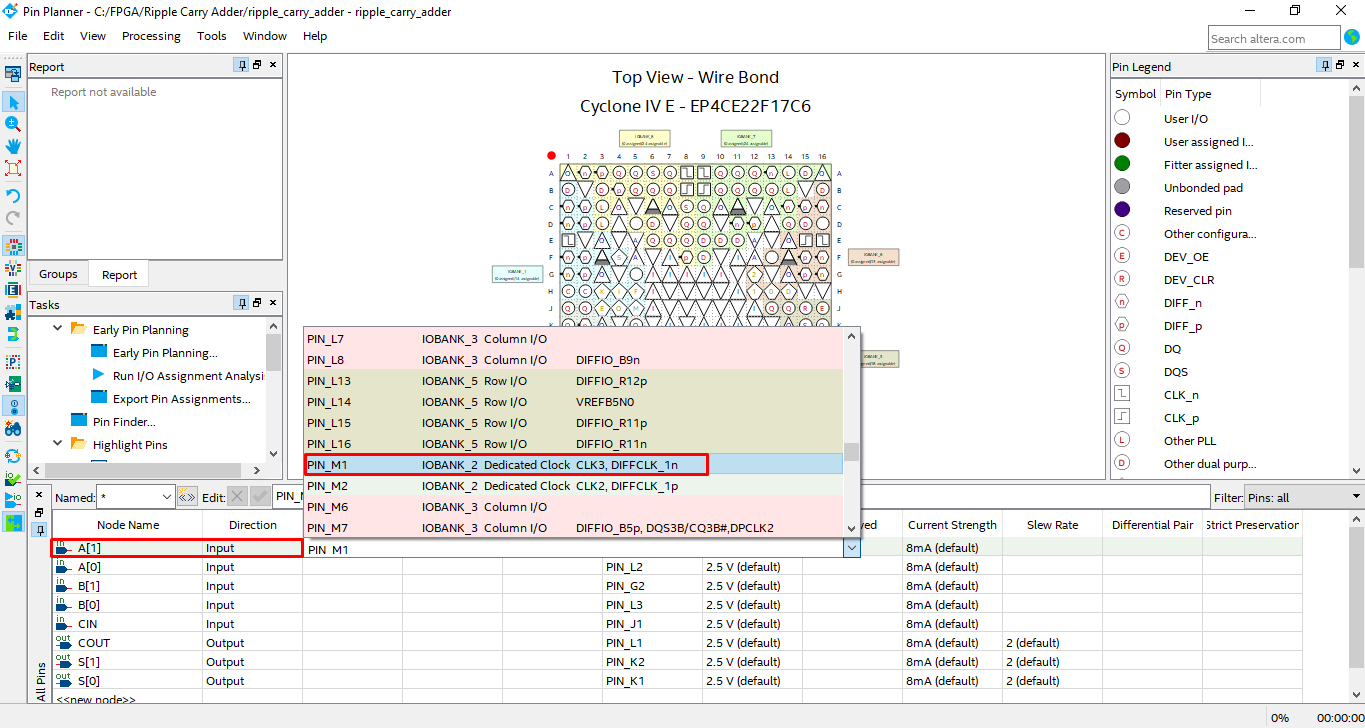
\includegraphics[height = 10cm, width = 15cm]{img for 3.2/img13.png}
\end{figure}
\noindent \textbf{Step 6}:You can use the Pin Tool for assigning I/O ports
\begin{figure}[H]
\centering
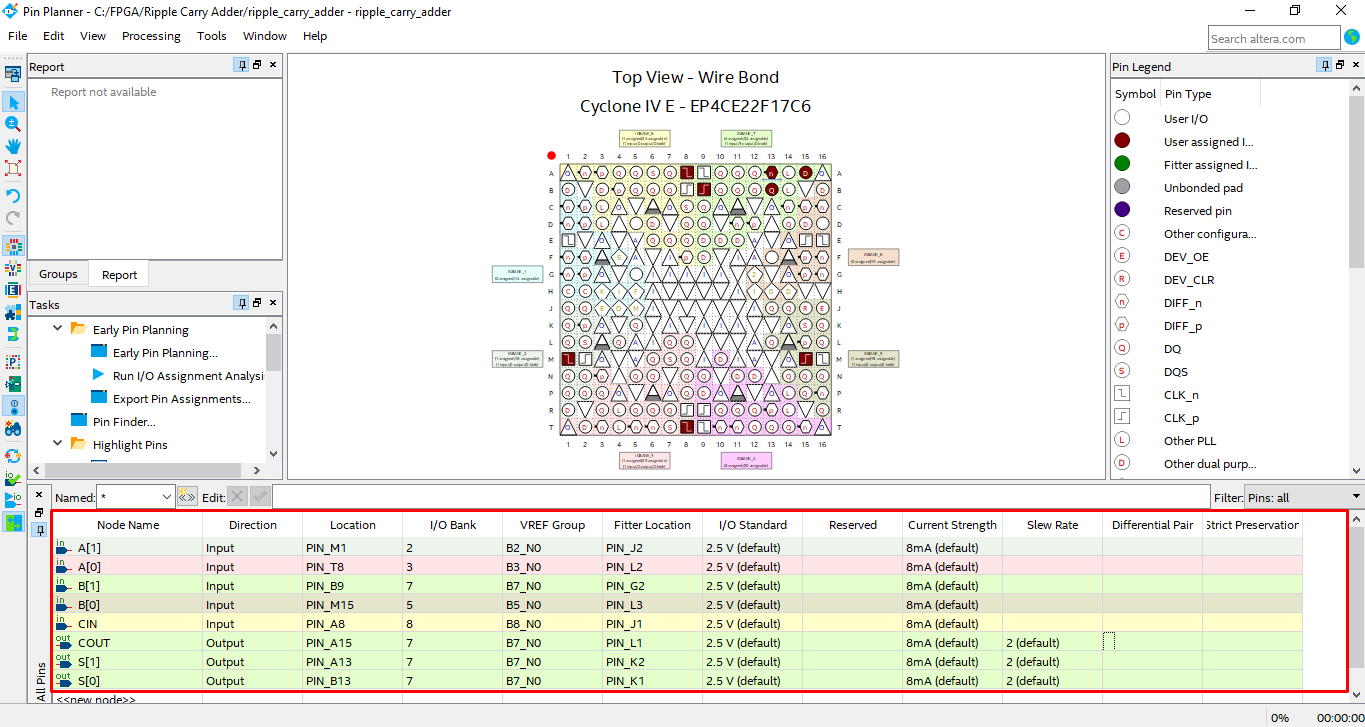
\includegraphics[height = 10cm, width = 15cm]{img for 3.2/img14.png}
\end{figure}
\noindent \textbf{Step 7}:To save the file, click on File$\rightarrow$Save as... Enter the name of your file and click on save.
\begin{figure}[H]
\centering
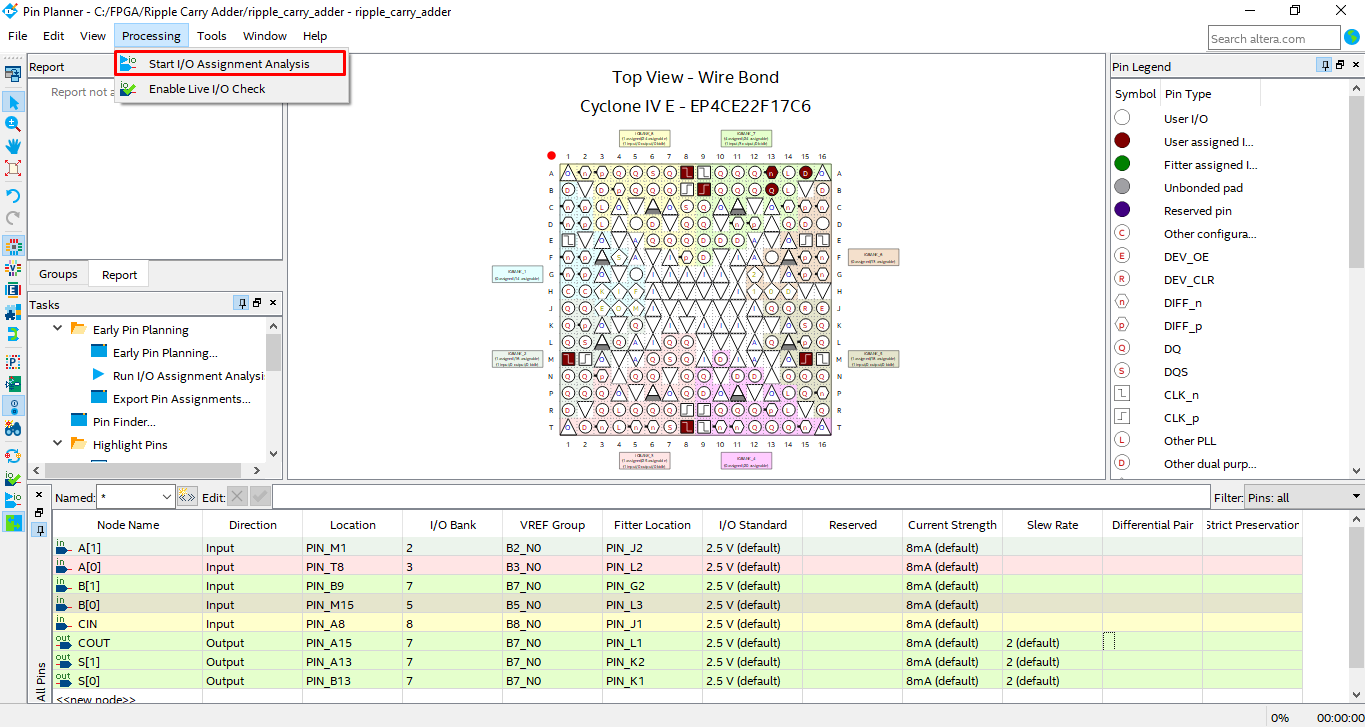
\includegraphics[height = 9cm, width = 15cm]{img for 3.2/img15.png}
\end{figure}
\end{enumerate}

%%%%%%%%%%%%%%%%%%%%%%%%%%%%%%%%%%%%%%%%%%%%%%%%%%%%%%%%%%%%%

\subsection{Compiling the project files}
\noindent \textbf{Step 1}:From the project navigator select the files option
\begin{figure}[H]
\centering
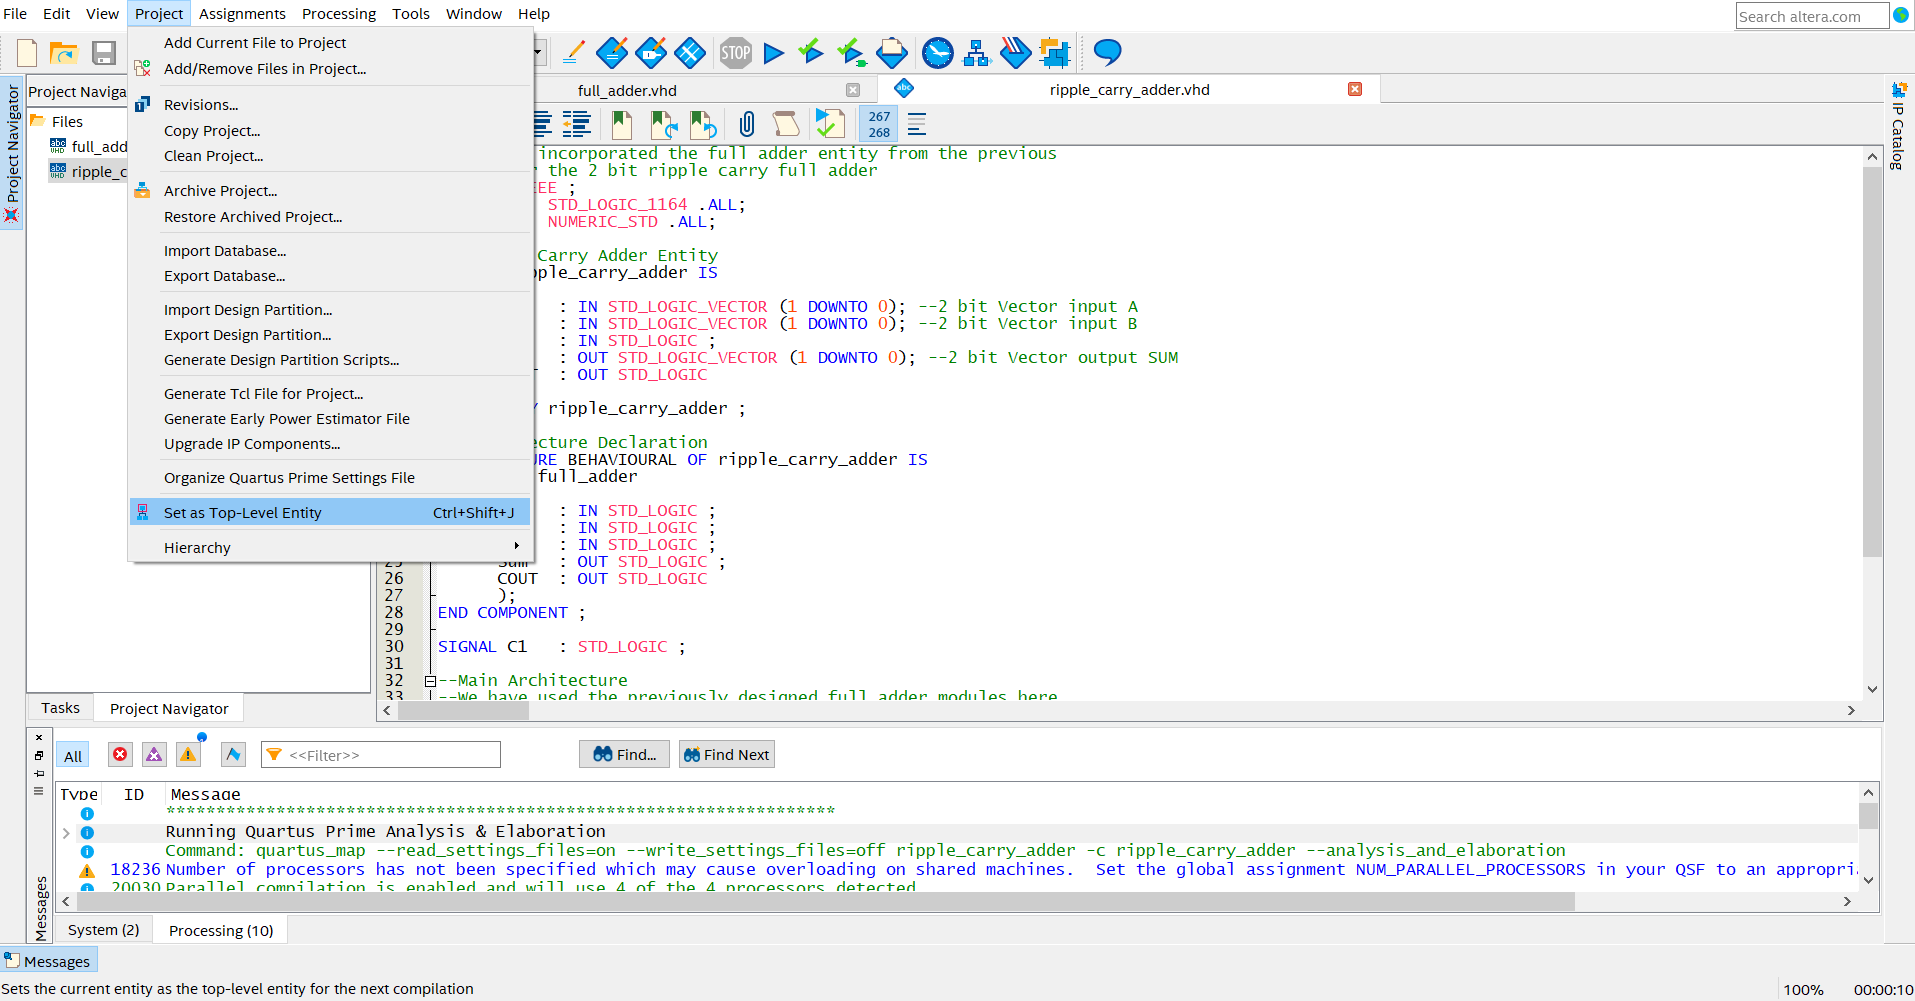
\includegraphics[height = 10cm, width = 15cm]{img_for_3.3/img6.png}
\end{figure}

\noindent \textbf{Step 2}:Right click on your verilog/VHDL file and select 'set as top level entity' option
\begin{figure}[H]
\centering
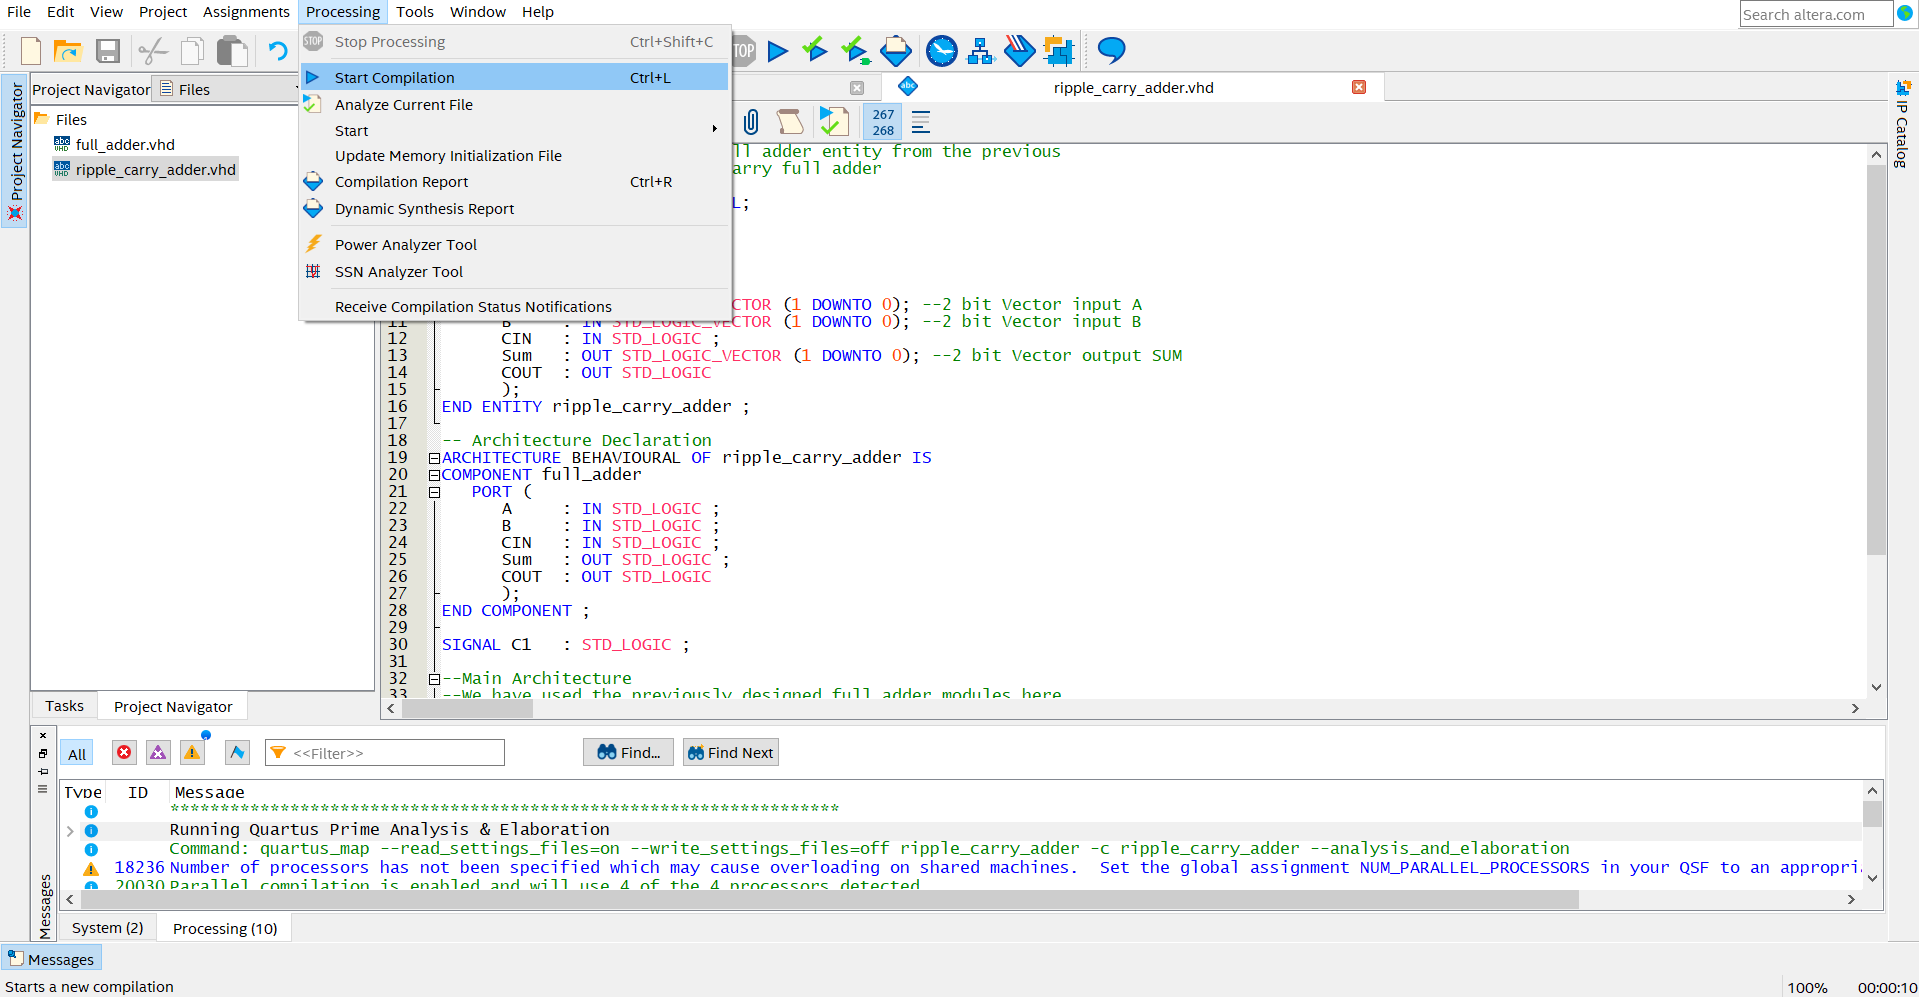
\includegraphics[height = 9cm, width = 15cm]{img_for_3.3/img7.png}
\end{figure}

\noindent \textbf{Step 3}: Go to processing and select 'start compilation' option
\begin{figure}[H]
\centering
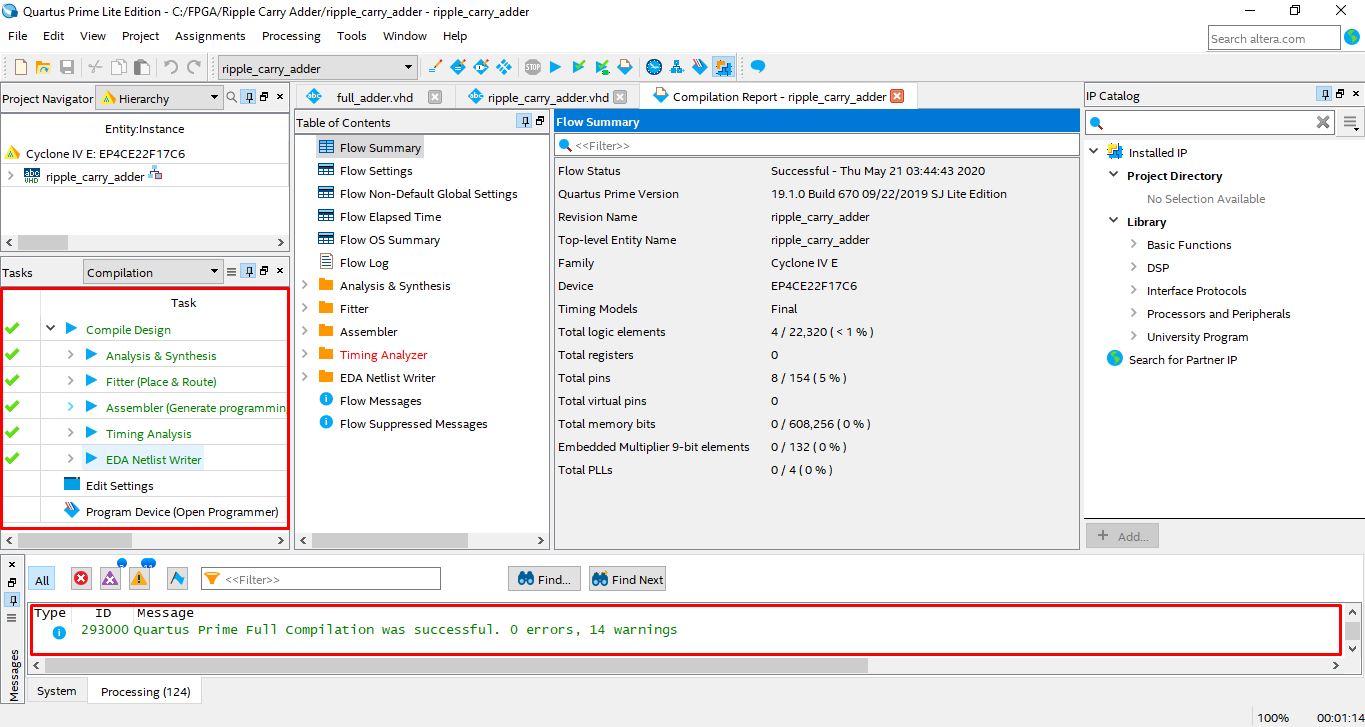
\includegraphics[height = 9cm, width = 15cm]{img_for_3.3/img8.png}
\end{figure}


%\--------------------------------------------------------------------------------



%\--------------------------------------------------------------------------------

\section{Verification by simulation(using ModelSim)}
\subsection{Without TestBench}
\noindent \textbf{Step 1}: Click on file and then click on New. From the list, Choose University Program VWF
\begin{figure}[H]
\centering
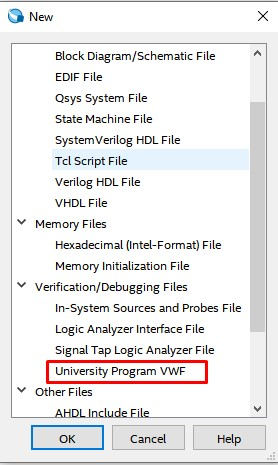
\includegraphics[scale=0.7]{Simulation_without_tb/first.jpg}
\end{figure}

\noindent \textbf{Step 2}: In the New window, Go to Edit$\rightarrow$Insert$\rightarrow$Node or bus
\begin{figure}[H]
\centering
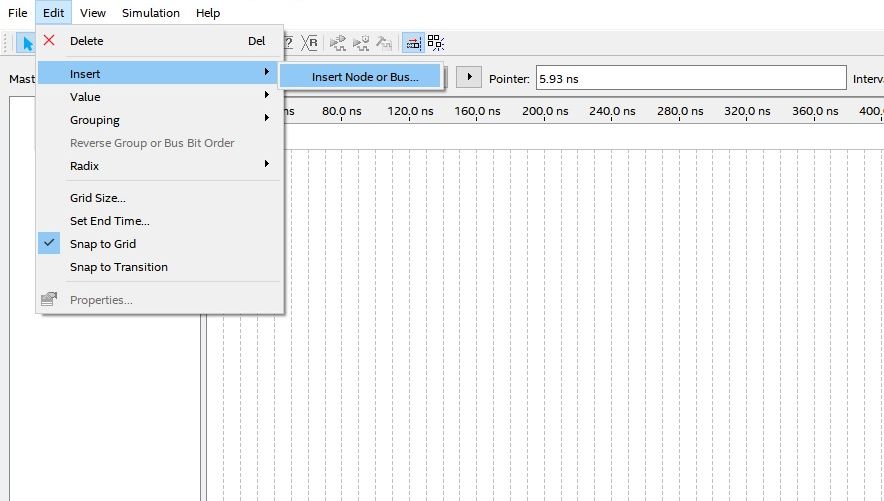
\includegraphics[scale=0.7]{Simulation_without_tb/second.jpg}
\end{figure}

\noindent \textbf{Step 3}: Click on Node Finder, in the new window, click on list
\begin{figure}[H]
\centering
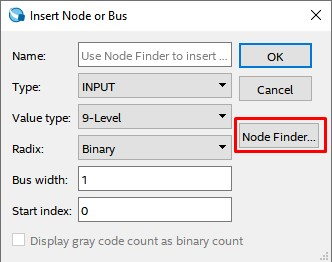
\includegraphics[scale=0.7]{Simulation_without_tb/third.jpg}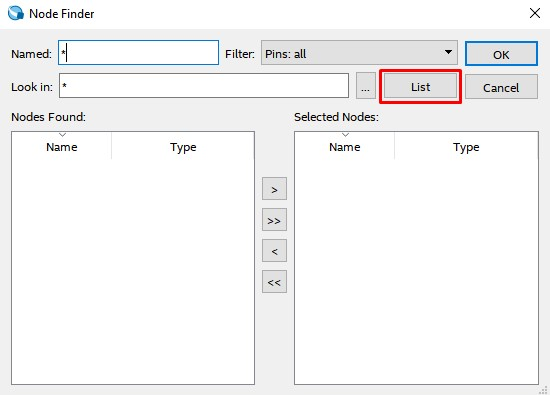
\includegraphics[scale=0.7]{Simulation_without_tb/third_1.jpg}
\end{figure}

\noindent \textbf{Step 4}: Click on the highlighted button to add all the Nodes. Now click on 'OK' and then 'OK' \hspace*{37pt} again
\begin{figure}[H]
\centering
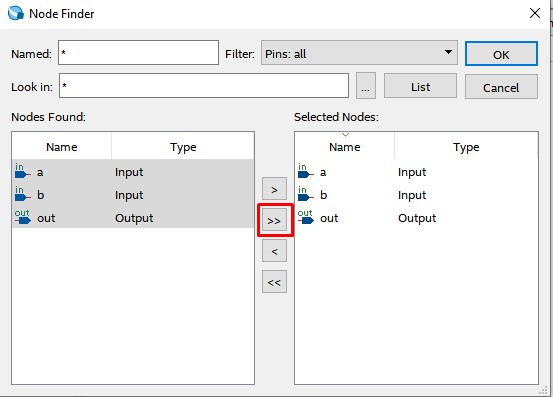
\includegraphics[scale=0.7]{Simulation_without_tb/fourth.jpg}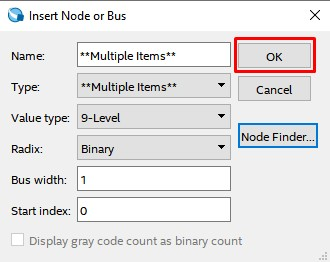
\includegraphics[scale=0.7]{Simulation_without_tb/fourth_1.jpg}
\end{figure}

\newpage
\noindent \textbf{Step 5}: Choose any of the input node and specify its value by choosing any of the options that \hspace*{39pt}are highlighted
\begin{figure}[H]
\centering
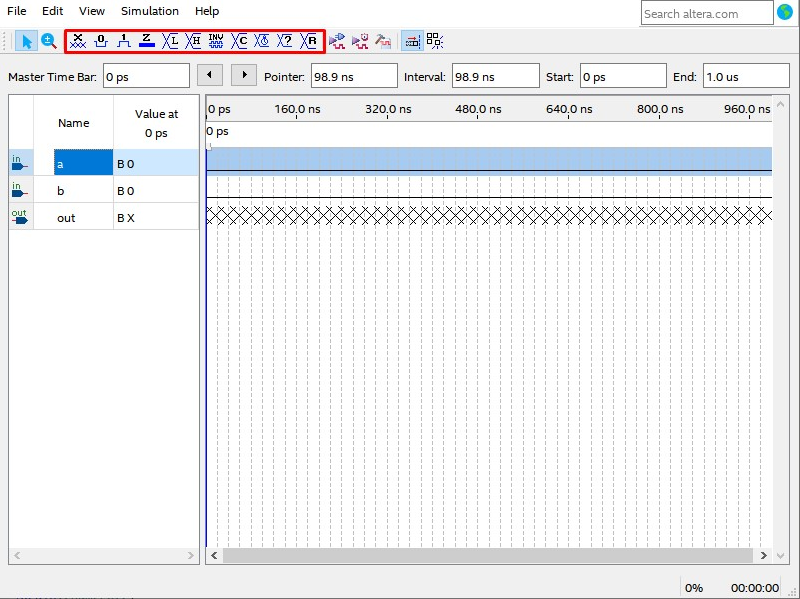
\includegraphics[height=10cm,width=15cm]{Simulation_without_tb/fifth.jpg}
\end{figure}

\noindent \textbf{Step 6}:For example, to give the alternating 'a' input, we first select the a node, then click on the \hspace*{35pt} count input type, and then specify the transition interval
\begin{figure}[H]
\centering
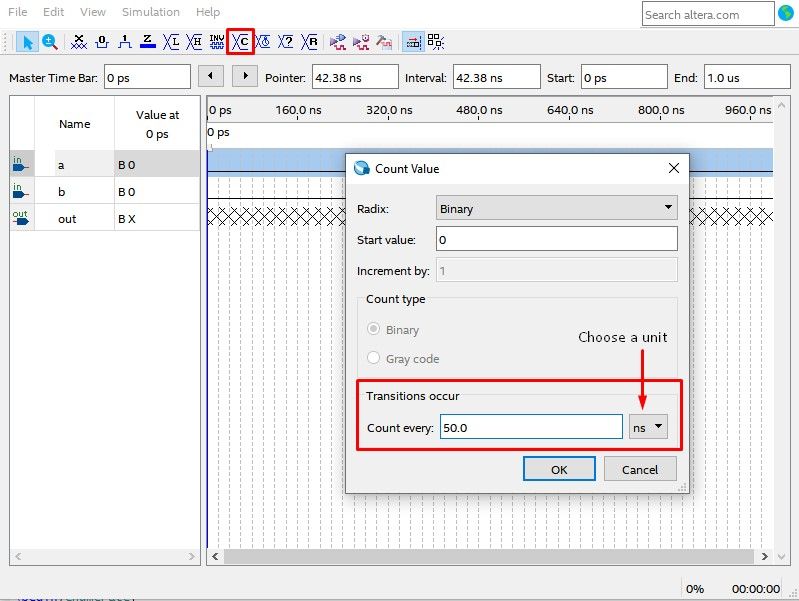
\includegraphics[height=9cm,width=17cm]{Simulation_without_tb/sixth.jpg}
\end{figure}

\newpage
\noindent \textbf{Step 7}:Similarly, specify the input patterns for all the inputs and then click on the simulate \hspace*{37pt}icon. If a save prompt appears, then save the file with a user defined name. Once the \hspace*{37pt}simulation process completes, the waveform will be displayed
\begin{figure}[H]
\centering
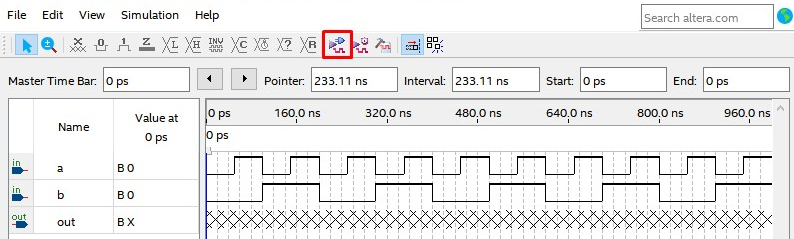
\includegraphics[scale = 0.8]{Simulation_without_tb/seventh.jpg}
\end{figure}
\begin{figure}[H]
\centering
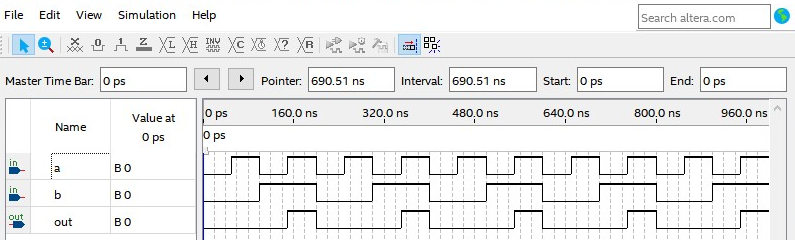
\includegraphics[scale = 0.6]{Simulation_without_tb/seventh_1.jpg}
\end{figure}

\newpage


% native link


\subsection{With Testbench and NativeLink}
\par\hspace*{20pt} Altera Quartus II software allows the user to launch                       Modelsim-Altera simulator from within the software using the Quartus             II feature called NativeLink. It facilitates the process of                     simulation by providing an easy to use mechanism and precompiled                 libraries for simulation.

\vspace{4mm}\noindent \textbf{Step 1} : Create a new verilog/VHDL file ,Add the testbench code and save it in the same \hspace*{37pt}project directory.\newline

    \begin{figure}[H]
    \centering
    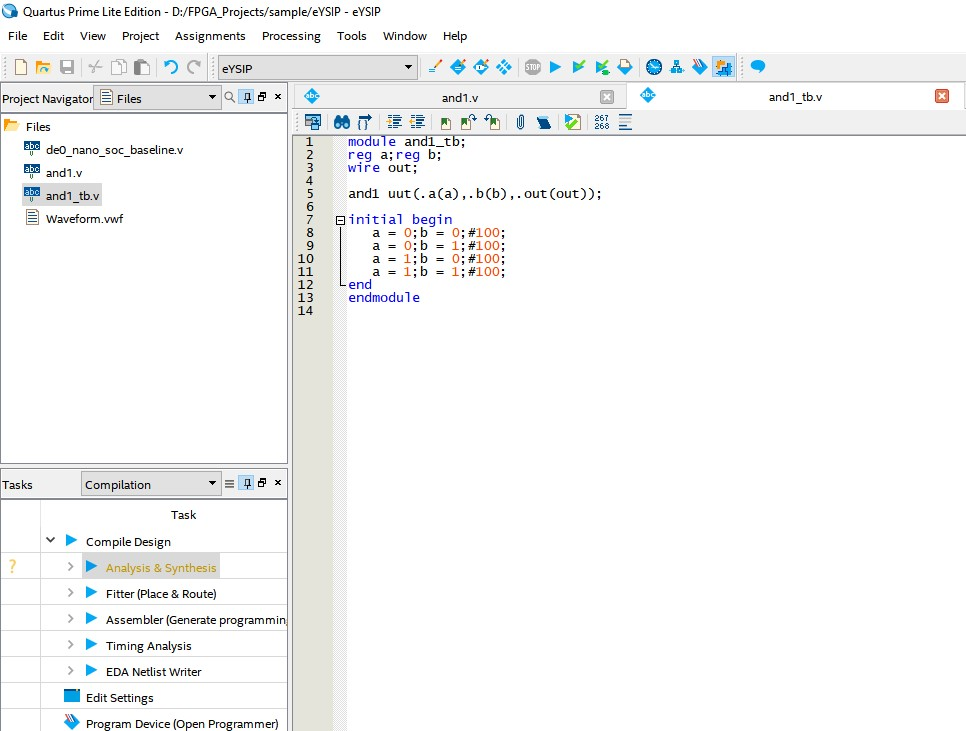
\includegraphics[scale=0.6,keepaspectratio]{nativelink/testbench1.jpg}
    \end{figure}
\noindent Testbench code for an AND gate:\newline

\noindent module and1\_tb;\newline
reg a;reg b;\newline
wire out;\newline

\noindent and1 uut(.a(a),.b(b),.out(out));\newline

\noindent initial begin\newline

	a = 0;b = 0;\#100;\newline
\hspace*{14pt}	a = 0;b = 1;\#100;\newline
\hspace*{14pt}	a = 1;b = 0;\#100;\newline
\hspace*{14pt}	a = 1;b = 1;\#100;\newline
	
\noindent end \newline
\noindent endmodule


\noindent \textbf{Step 2}: \underline {Specify the path to Modelsim Altera:}
\begin{enumerate}
    \item Go to the menu Tools $\rightarrow$ Options
    \item In the 'General' category, select 'EDA Tool Options'.
    %\newpage 
    \item A dialogue box appears, where you can specify the location path of the Modelsim-Altera   \hspace*{5pt} executable file.And click 'OK'.
            \begin{figure}[H]
                \centering
                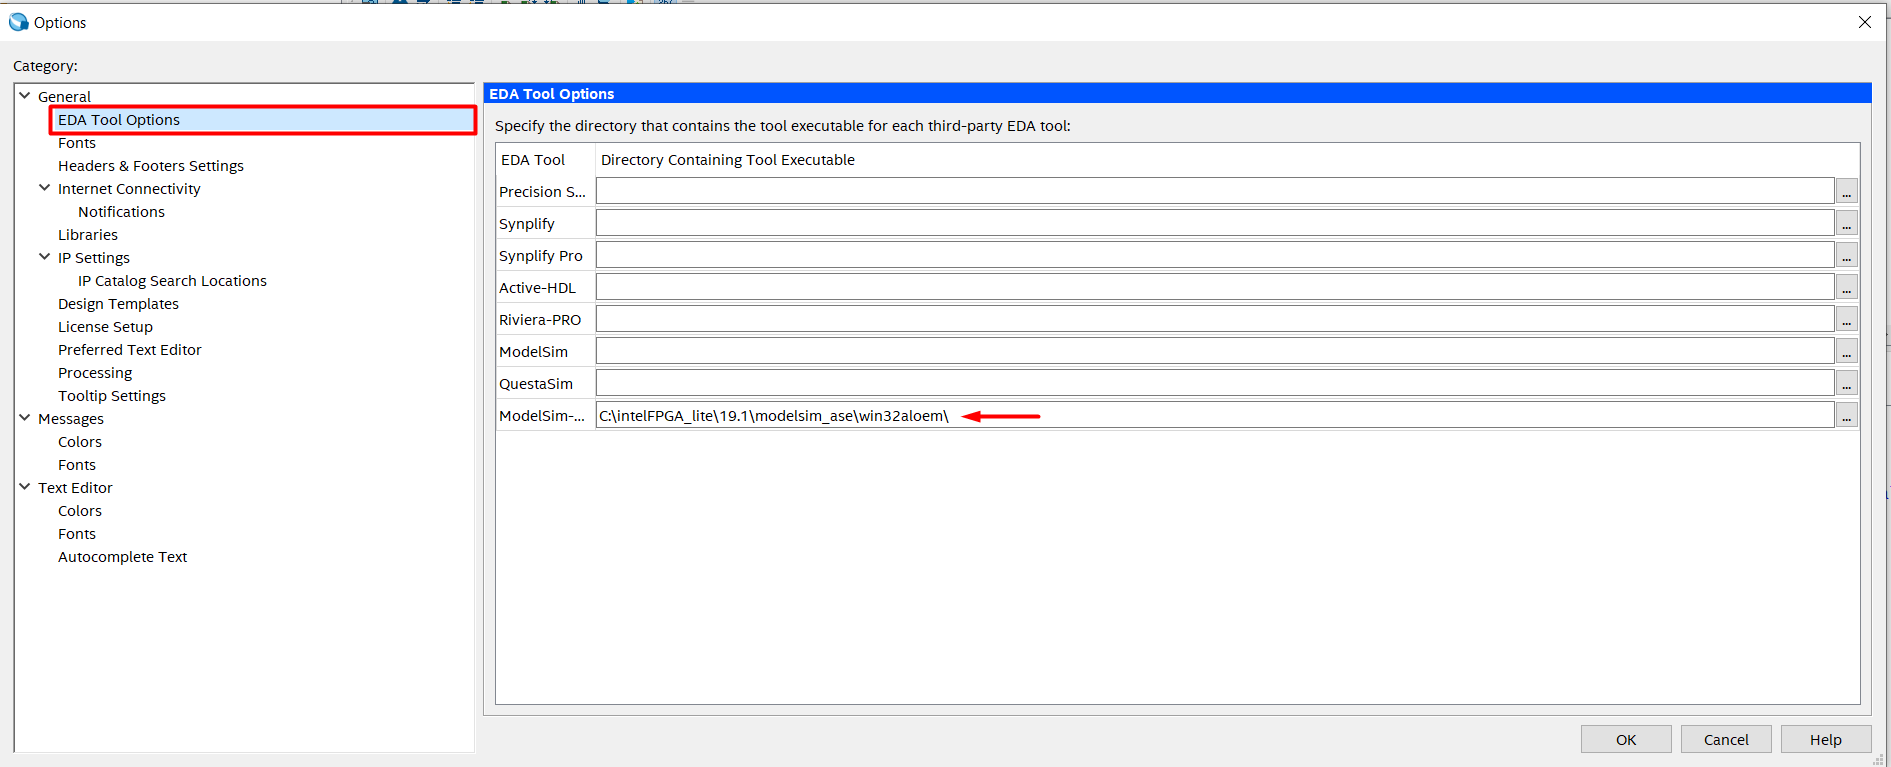
\includegraphics[scale=0.8]{nativelink/nativelink_1.png}
            \end{figure}
          
\end{enumerate}
\vspace{5mm}


\noindent \textbf{Step 3} : \underline{ NativeLink Settings to configure Modelsim-Altera:}
\begin{enumerate}
    \item Go to the menu Assignments $\rightarrow$ Settings.
    \item Under 'EDA Tool Settings' choose 'Simulation'. The dialogue box for
           simulation appears.
    \item For Tool Name, choose 'Modelsim-Altera'.
    \item Select 'VHDL'(or Verilog/systemVerilog) as the 'Format for Output Netlist'.
    \item Select 'simulation/modelsim' as the 'Output Directory.
    \item Under NativeLink Settings, Choose 'Compile test bench'. Then click on       'Test Benches'.All these changes are indicated in the below figure.
        \begin{figure}[H]
            \centering
            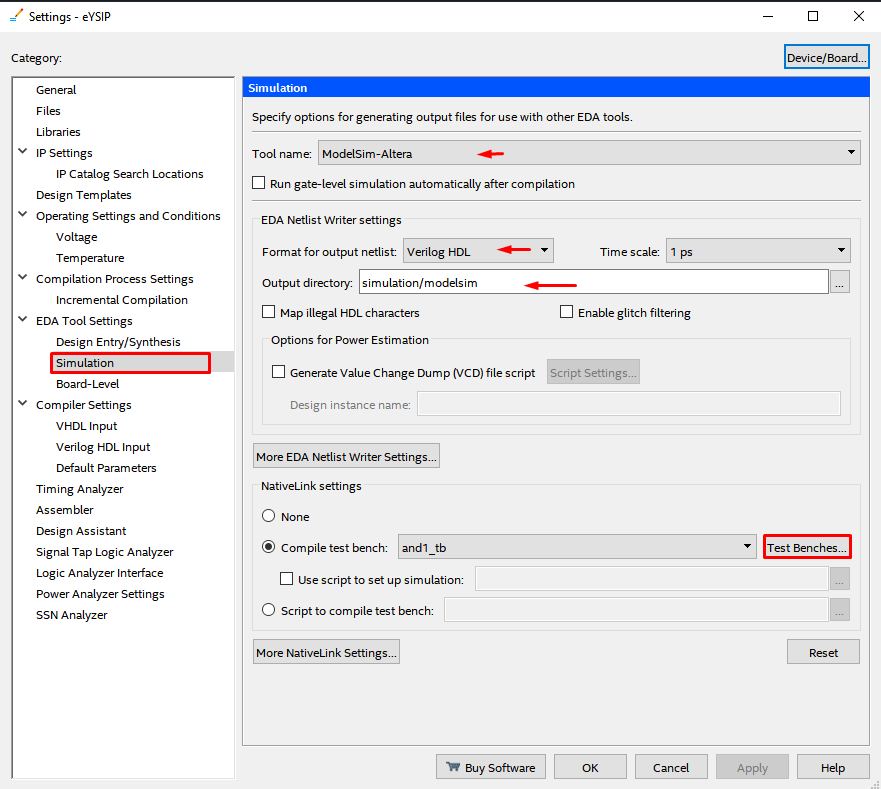
\includegraphics[scale=0.6]{nativelink/nativelink_2.png}
        \end{figure}
    \item A new window appears select 'New'
        \begin{figure}[H]
            \centering
            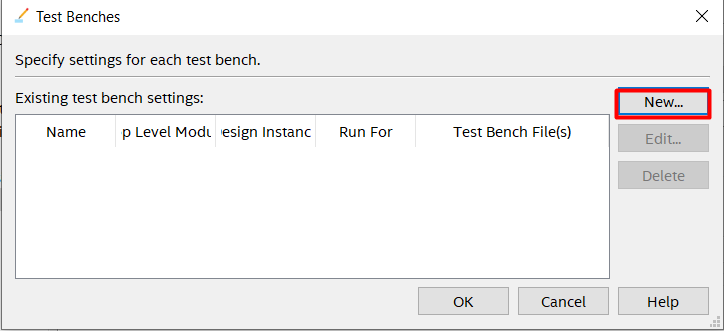
\includegraphics[scale=0.7]{nativelink/nativelink_3.png}
        \end{figure}
    \item Another window appears with the name 'New Test Bench Settings'.
    \item Enter the 'Test Bench Name' and 'Top Level Module in test bench'.
    \item Add the test bench file and then click 'OK'.
        \begin{figure}[H]
            \centering
            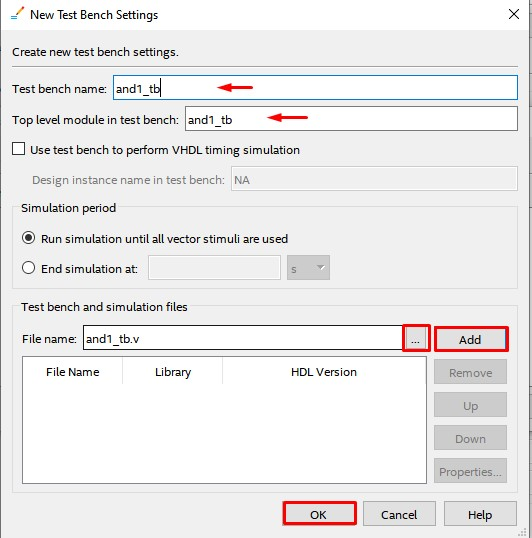
\includegraphics[scale=0.5]{nativelink/nativelinktestbench settings.jpg}
           
        \end{figure}
\end{enumerate}

\noindent \textbf{Step 4} : \underline{ Functional Simulation using NativeLink Feature:}
\begin{enumerate}
    \item Goto menu 'Processing', select 'Start', and then click 'Start Analysis \& Elaboration'.After this click on 'Start Analysis \& Synthesis 'on the same drop box .These step checks the error and collects all file name information and builds the design hierarchy for simulation.
        \begin{figure}[H]
            \centering
            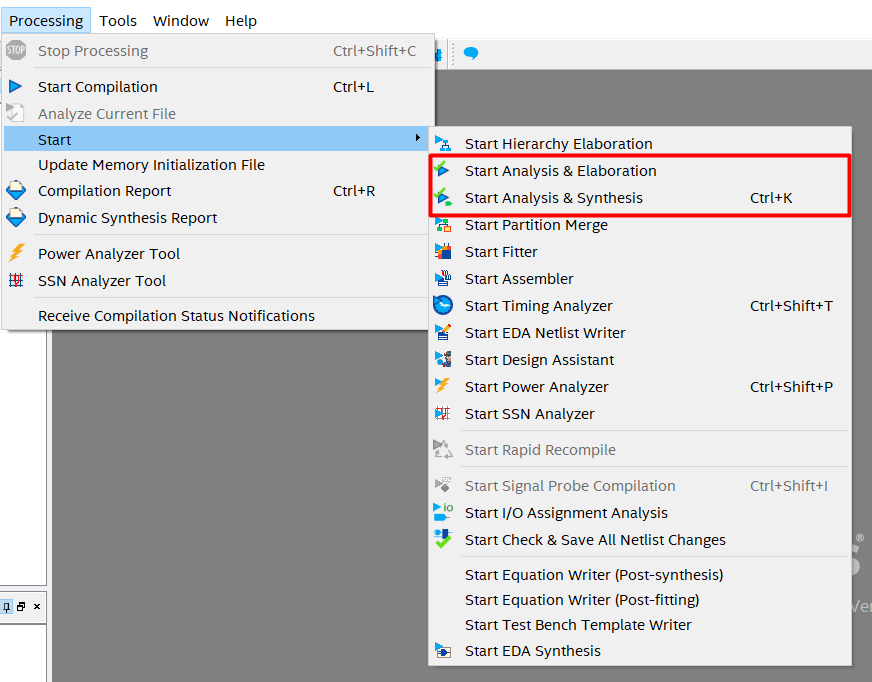
\includegraphics[height=10cm, width=15cm]{nativelink/new analyse.png}
        \end{figure}
    \newpage
    \item Goto menu 'Tools', click on 'Run Simulation Tool', and then click
         “RTL Simulation” to automatically run the EDA simulator(ModelSim-Altera) and to compile all necessary design files.
         \begin{figure}[H]
            \centering
            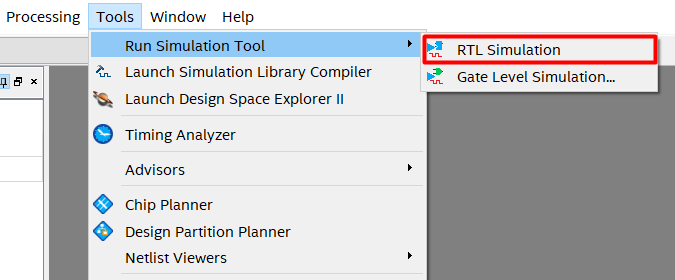
\includegraphics[scale=0.45]{nativelink/native link run.png}
        \end{figure}

    \item Finally ModelSim-Altera tool opens with simulated waveforms.
        \begin{figure}[H]
            \centering
            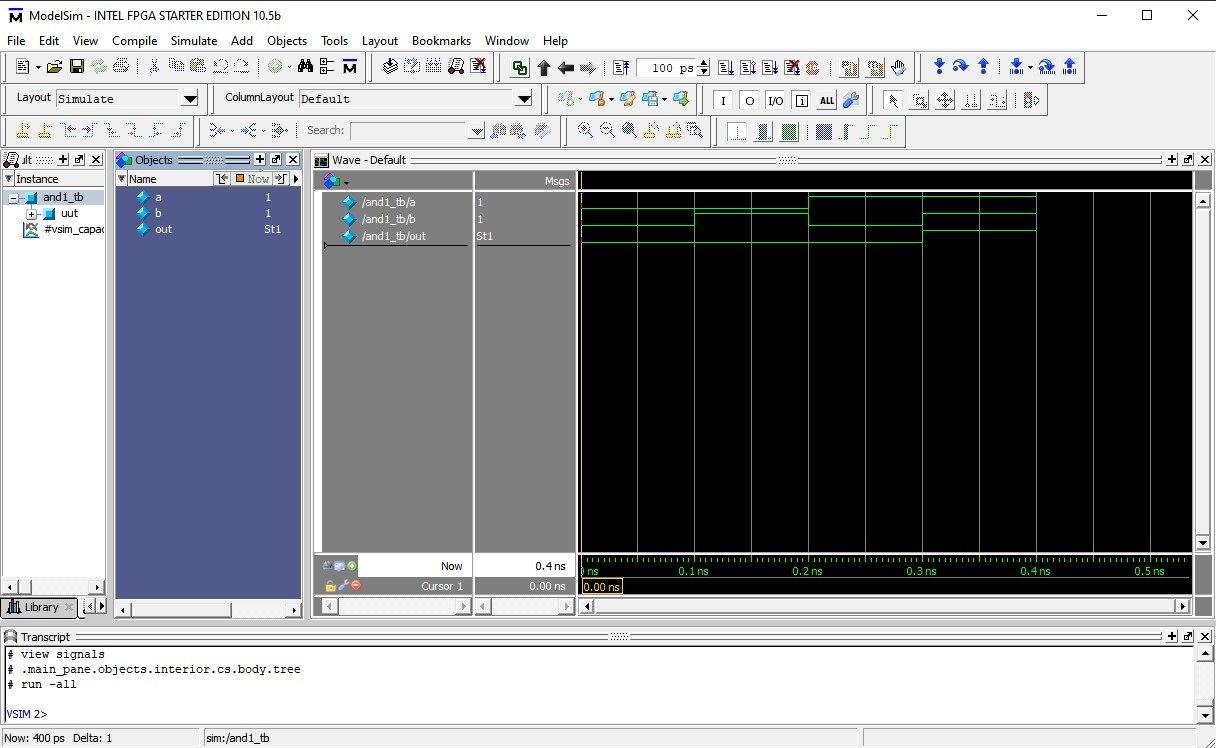
\includegraphics[scale=0.45]{nativelink/nativelink_waveform.jpg}
           
        \end{figure}
\end{enumerate}

%\---------------------------------------------------------------------------
\section{Timing Analysis using TimeQuest}

%\-----
\subsection{Introduction to timing analysis}

\par 
The process of analyzing delays of a logic circuit to determine the condition under which the given circuit operates reliably is known as Timing Analysis.
It can be used to calculate delay for every possible logical path in the design. It can also be used to determine the maximum operational frequency for the circuit.
\\
We can use Timing Analyzer in Quartus to perform a detailed analysis of our FPGA design. This ensures that the specified timing constraints were properly passed to the implementation tools. 

%\-----

\subsection{Creating a Synopsis Design Constraints file}
Now that we know the importance and what actually timing analysis,let’s create a Synopsis Design Constraints or an SDC file and then we have to add it to our project as the main timing constraints file. \\
To create a new *.sdc file
\begin{enumerate}
    \item Click on New file under the File menu
    \item Select the Synopsis Design Constraints File from under the Other Files section.
        \begin{figure}[H]
            \centering
            \includegraphics[scale=0.7]{TimingAnalysis/timing1.png}
        \end{figure}
        
     \item Click ok then save this file with the same name as our top-level entity file name 
     So that this file will include in the main compilation process automatically, you can name the file differently but then you have to manual add it to Settings page.
     \begin{figure}[H]
            \centering
            \includegraphics[scale=0.5]{TimingAnalysis/timing2.png}
        \end{figure}
\end{enumerate}

\subsection{Adding Timing Constraints}
Adding a time constrainst is a necessary step but simple design doesn't require timing constraint but it is recommended to add one to avoid unnecessary warning message from our compilation process.
\\
To add a timing constraint follow the steps
\begin{enumerate}
    \item Clicking on Insert Constraint under the Edit menu.
    \begin{figure}[H]
            \centering
            \includegraphics[scale=0.4]{TimingAnalysis/timing3.png}
        \end{figure}
        
      \item There are various types of constraints that could be used in our design, because all the timing related activities involves a clock.\\
      To create a clock for timing analysis, Select Create Clock from within Insert Constraint ​under the Edit menu.
      \begin{figure}[H]
            \centering
            \includegraphics[scale=0.7]{TimingAnalysis/timing4.png}
        \end{figure}
        
        Enter the clock frequency in the period section, for example for a 50MHz clock period is 20ns.Then Click on Insert.
        
        \item Insert Constraint again and this time select Derive PLL Clocks to generate a constraint for the PLL clock that has been derived from our main input clock. Uncheck the box as shown in the figure
        \begin{figure}[H]
            \centering
            \includegraphics[scale=0.8]{TimingAnalysis/timing5.png}
        \end{figure}
        
        
        \item Insert Constraint again and this time select Derive Clock Uncertainty and save the file. 
​       \begin{figure}[H]
            \centering
            \includegraphics[scale=0.9]{TimingAnalysis/timing6.png}
        \end{figure}
        \begin{figure}[H]
            \centering
            \includegraphics[scale=0.35]{TimingAnalysis/timing7.png}
        \end{figure}
    
\end{enumerate}

\subsection{Running Full Compilation and TimeQuest Analysis}

Now all the steps to set timing constraint are done. Now we can run the full compilation process. This can be done by clicking on
        \begin{figure}[H]
            \centering
            \includegraphics[scale=0.4]{TimingAnalysis/timing8.png}
        \end{figure}\\
        
        This step can take some time depending upon the complexity of your design and your system specification.
        \begin{figure}[H]
            \centering
            \includegraphics[scale=0.35]{TimingAnalysis/timing9.png}
        \end{figure}\\
        
TimeQuest Timing Analysis uses Synopsis Design Constraint timing analysis file that we just created to generate a report.
To start analysis click on the Timing Analyzer in table of content then click on the clocks and then right click on the clock on which analysis has to be done and select Report Timing (in Timinng Analyzer UI)    
        \begin{figure}[H]
            \centering
            \includegraphics[scale=0.45]{TimingAnalysis/timing10.png}
        \end{figure}\\

\end{document}
